\documentclass[landscape,a0,final]{a0poster}
\usepackage[dvipsnames,svgnames]{xcolor}
\usepackage{tikzposter} % here most of the things are defined
% change parameters only after this line You can also start a new column with an arbitrary 
% x-coordinate by specifying explicitly the coordinate of the new block node as follows:
\usepackage[czech]{babel}
\usepackage[utf8]{inputenc}
\usepackage{wrapfig}
\usepackage{url}

% For blibliography styling
\usepackage{natbib}

%Used for better control on code display

\usepackage[margin=\margin cm, paperwidth=197cm, paperheight=100cm]{geometry}

% \setbackgrounddarkcolor{ForestGreen!70!black}
% \setbackgroundlightcolor{YellowGreen!90!}

% \setfirstcolor{YellowGreen!80!}
% \setsecondcolor{gray!80!}
% \setthirdcolor{red!80!black}

\title{Improving the Apollo 12 landing site mapping\\with Chandrayaan $M^3$ data}
\author{Yann Chemin$^{1,2}$, Ian Crawford$^1$, Roberto Bugiolacchi$^1$, Huma Irfan$^1$ and Louise Alexander$^1$\\
$^1$Birkbeck College, University of London, U.K. ~ $^2$IWMI, Pelawatte, Sri Lanka}

\usetemplate{1}
\setinstituteshift{1}

\setblocktitleheight{2}
\setblockspacing{1}

\begin{document}
\ClearShipoutPicture
\AddToShipoutPicture{\BackgroundPicture}
\noindent
\tikzstyle{every picture}+=[remember picture]
\begin{tikzpicture}
\initializesizeandshifts
\titleblock{90}{1}
% \setblocktitleheight{1}

%\addlogo[north west]{(2,-1)}{9cm}{./svg_images/Grass_GIS.pdf}
%\addlogo[north east]{(-2,-2.5)}{11cm}{./svg_images/IWMI_logo.pdf}

%%%%%%%%%%%%%%%%%%%%%%%%%%%%%%%%%%%%%%%%%%%%%%%%%%%%%%%%%%%%%%%%%%%%%%%%%%%%%%%%
\blocknode{Abstract}{
\small \noindent The geology of the Apollo 12 landing site has been the subject of many studies, including recently by \cite{korotev2011apollo} and \cite{Snape2013basaltic}. This research attempts to bring additional understanding from a remote sensing perspective using the Moon Mineralogy Mapper ($M^3$) sensor data, onboard the Chandrayaan lunar orbiter. This has a higher spatial-spectral resolution sensor than the Clementine UV-Vis sensor and provides the opportunity to study the lunar surface with detailed spectral signatures.\vspace{5mm}\newline
Mapping of FeO (wt\%) and TiO 2 (wt\%) is done using the methods of \cite{lucey2000lunar} and \cite{wilcox2005mapping}. A FeO \& TiO 2 processing module (i.feotio2) is made specifically for this research within the Free \& Open Source Software GRASS GIS \cite{neteler2012grass}. Attempts will be made to estimate the lava flow thickness using the method of \cite{bugiolacchi2006stratigraphy} and individual lava layers thicknesses from \cite{weider2010individual}. Integration of this new information will be put in perspective and integrated with previous work. Analysis from the combined higher spatial and spectral resolutions will improve the accuracy of the geological mapping at the Apollo 12 landing site.
}


%%%%%%%%%%%%%%%%%%%%%%%%%%%%%%%%%%%%%%%%%%%%%%%%%%%%%%%%%%%%%%%%%%%%%%%%%%%%%%%%
\blocknode{Previous interpretations}{
\cite{korotev2011apollo} reviewed the lunar research done until recently, with a special interest in the Apollo 12 landing site and its vicinity. Among the information newly deducted, are a geological context block diagram 1 (Figure below) along with an Apollo 12 landing site interpretive cross-section. \cite{fortezzo2013completed} completed the digital renovation of the 1:5,000,000 lunar geological maps series, enhanced with LOLA-LRO information.
\begin{center}
	\begin{tabular}{cc}
		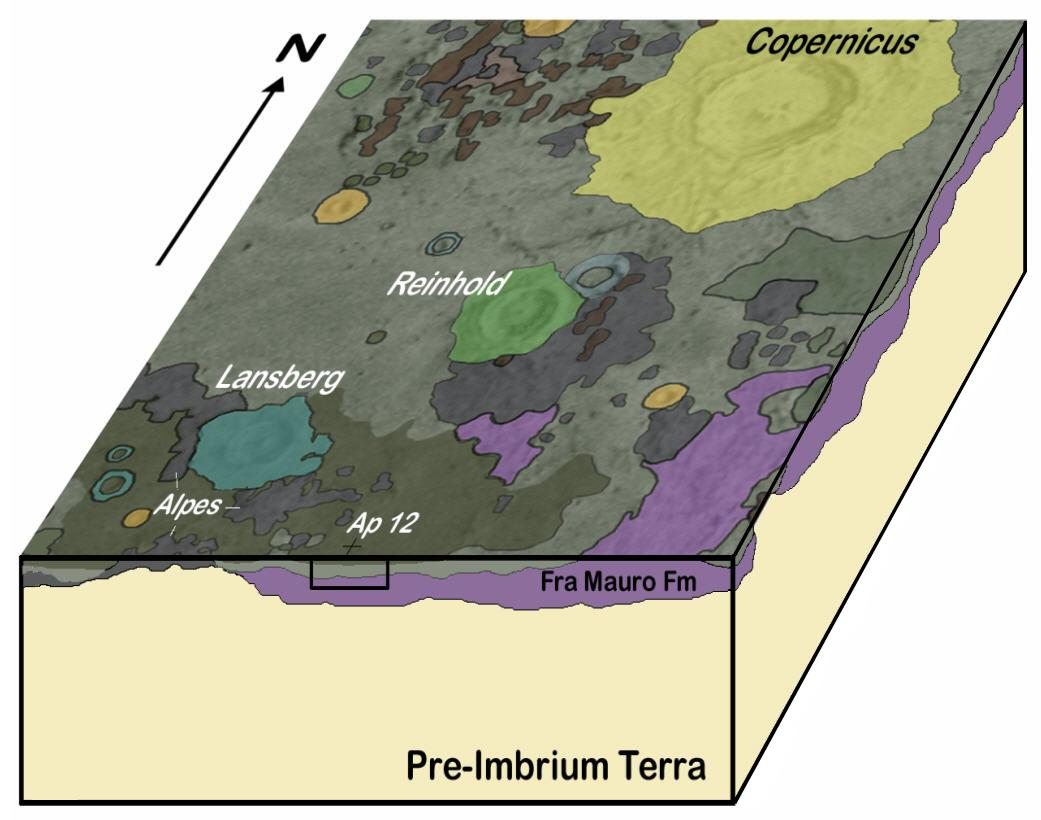
\includegraphics[width=0.45\textwidth]{./images/Korotev_block}\hspace{20mm}
		&
		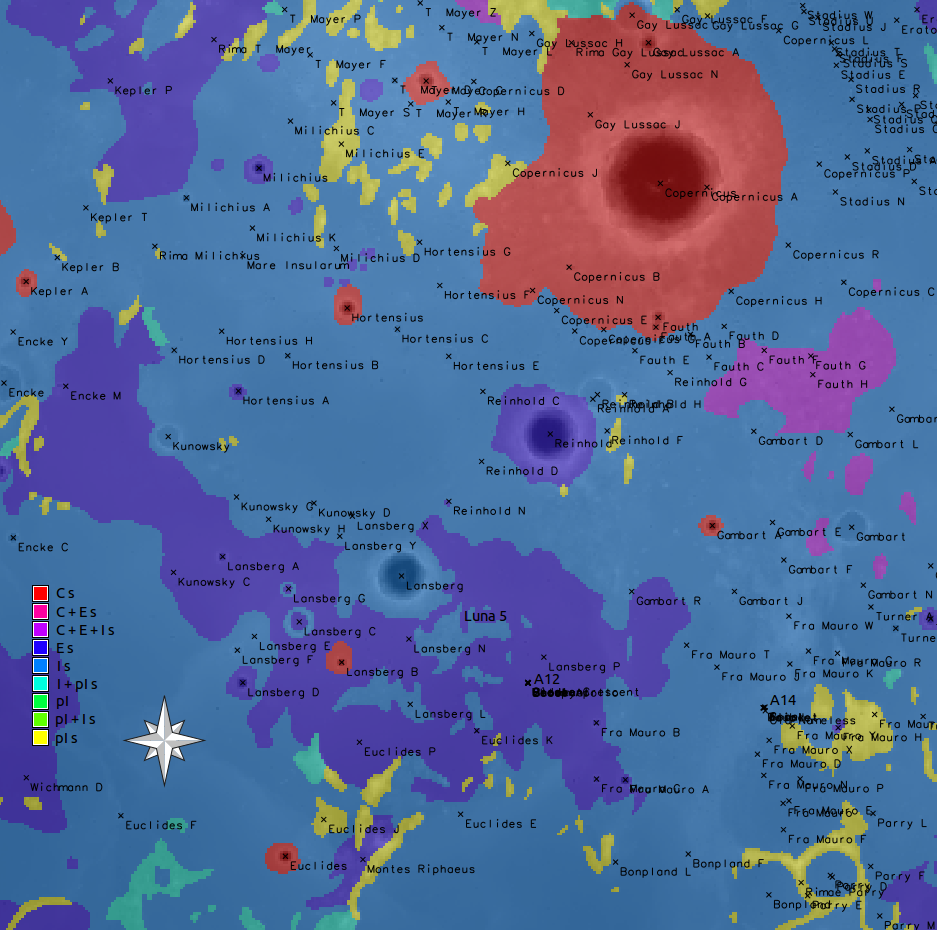
\includegraphics[width=0.45\textwidth]{./images/A12region}
	\end{tabular}\newline
Figure 1: a) Geological block of Apollo 12 landing site from \cite{korotev2011apollo}.\\
b) Geological maps series with moon nomenclature from \cite{fortezzo2013completed}.
\end{center}

\begin{center}
	\begin{tabular}{c}
		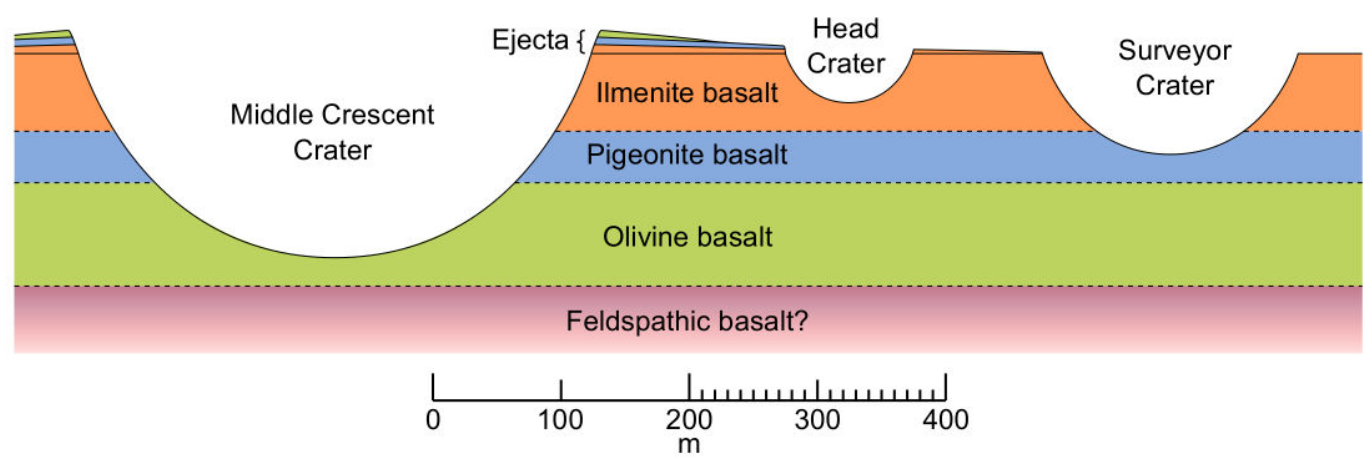
\includegraphics[width=0.75\textwidth]{./images/2013_lpsc_Snape_et_al}
	\end{tabular}\newline
Figure 2: Interpretive cross-section of Apollo 12 landing site from \cite{Snape2013basaltic}. 
\end{center}
}


%%%%%%%%%%%%%%%%%%%%%%%%%%%%%%%%%%%%%%%%%%%%%%%%%%%%%%%%%%%%%%%%%%%%%%%%%%%%%%%%
%\getcurrentrow{box}
%\coordinate (funkcionalita) at (box.south west);
%\coordinate (funkcionalitaeast) at (box.east);
%\coordinate (screenshot) at (box.north west);
%
%\blocknodew[($(funkcionalita)+(20,-1)$)]{35}{References}{
\blocknode{References}{
\smallskip
\scriptsize

\begingroup
\renewcommand{\section}[2]{}%
\bibliographystyle{plain}
\bibliography{poster}
\endgroup

%\hrulefill
%\vspace{-5pt}

\begin{center}
\begin{tabular}{c}
\hspace{5mm}
\begin{minipage}{0.2\textwidth}

\includegraphics[width=0.5in]{./images/grass_qr.pdf}
\end{minipage}

\begin{minipage}{0.25\textwidth}
\small {\url{www.bbk.ac.uk}}
\end{minipage}

\begin{minipage}{0.15\textwidth}

\includegraphics[width=0.7in]{./svg_images/public_domain_logo.pdf}
\end{minipage}

\begin{minipage}{0.3\textwidth}
\small {\url{grass.osgeo.org}}
\end{minipage}

\begin{minipage}{0.2\textwidth}

\includegraphics[width=0.5in]{./images/grass_qr.pdf}
\end{minipage}

\end{tabular}
\end{center}

}

\startsecondcolumn

%%%%%%%%%%%%%%%%%%%%%%%%%%%%%%%%%%%%%%%%%%%%%%%%%%%%%%%%%%%%%%%%%%%%%%%%%%%%%%%%
\blocknode{M$^3$ derived FeO from standard equations}{
\bigskip

\begin{center}
\begin{tabular}{ c p{0.45\textwidth}}
 \raisebox{-1.1\totalheight}{\includegraphics[width=0.5\textwidth]{./code/code1.pdf}}
 %\caption{Testing FeO algorithms.}
 \label{fig:FeOtesting}
 &
\noindent The wt\%FeO equations have a large range of results when used with $M^3$ data:\newline
\begin{center}
\begin{tabular}{ l r r}
\hline
Authors & Bench & Surveyor\\
\hline
\cite{lucey2000lunar} & -26.64 & -23.32 \\
\cite{lawrence2002iron} & 4.72 & 6.38 \\
\cite{wilcox2005mapping} & 22.28 & 21.82 \\
\cite{zhang2013mapping} & 19.74 & 19.49 \\
\cite{zhang2013mapping} (corrected) & 15.65 & 14.76 \\
\hline
\end{tabular}
\end{center}
\bigskip
 \noindent It is known that the local range of FeO is below 10wt\% from UVVIS data (see Figure on the lower left), only the \cite{lawrence2002iron} equation is giving an appropriate range. \cite{lucey2000lunar} equation fails because of the offset of uvvis4/uvvis2(=1.15 vs offset = 1.19) and the one for uvvis2(=0.05 vs offset = 0.08), as both of the parts are negative thus giving a positive division output, their interplay should bring a negative number for the arctangent negative sign to compensate. This clearly does not happen with $M^3$ data in the Bench and Surveyor craters, the results from the arctangent being positive, and the sign change brings the main part of the equation to a negative, further reduced by the negative final offset.\newline
\end{tabular}
\end{center}
\noindent Upon using the equation from \cite{lawrence2002iron}, it turned out that though the wt\%FeO range was satisfactory for few crater points, the rate of change was actually reverse to the expected one, reducing to null towards the South of the landing site and increasing towards the North.\vspace{5mm}\newline
\noindent The equation from \cite{zhang2013mapping} is giving an appropriate rate of change, however, the local values are too large compared to the Clementine derived FeO values. Comparing the zonal contrast between Clementine FeO map from \cite{lucey2000lunar} the $M^3$ from \cite{zhang2013mapping} leads to an interesting prospect as even the shapes are not consistent (see Figures ~\ref{fig:subfeoclem} \& ~\ref{fig:subfeoM3}). This indicates that the inner work of the angle equation is not sensitive to the same type of distance between R950 and R750 as they are in Clementine and in $M^3$. In an ideal condition, the calibration of both sensor bands would be identical, and the sensor response for each band would also be the same. This is not a reality, from the design and manufacture inheritance of multi-spectral sensors and hyperspectral sensors, to the data collection flight and its environment. Finally, some accident or issues can damage the operation.\vspace{5mm}\newline
\noindent After Contacting W. Zhang of \citep{zhang2013mapping} about the issue in its algorithm, he promptly answered that the article had a typo in the equation. After correction, the output were in a better range (about 15 for the two craters in the table above).\newline

\begin{center}
\begin{tabular}{ c c }
 \raisebox{0.0\totalheight}{ 
 \begin{tabular}{ p{0.45\textwidth} }
  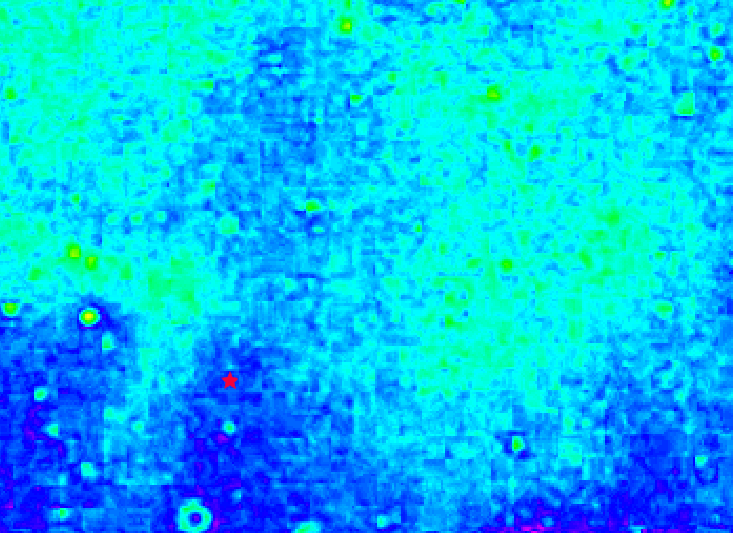
\includegraphics[width=0.45\textwidth,keepaspectratio=true]{./images/Clem_FeO_area}
% \caption{Subset of Clementine FeO using \citep{lucey2000lunar}}
 \label{fig:subfeoclem}
 Figure 4: Subset of Clementine FeO using \cite{lucey2000lunar}.
 \newline\linebreak
\vspace{10mm}\\
 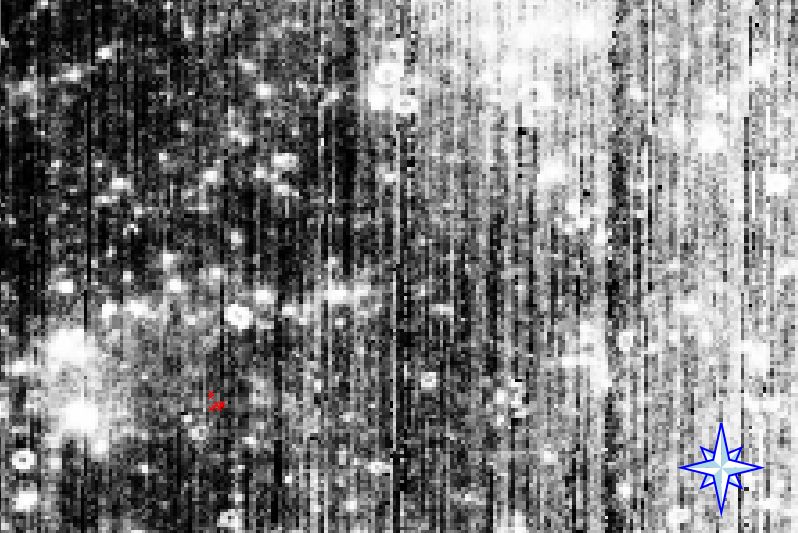
\includegraphics[width=0.45\textwidth,keepaspectratio=true]{./images/M3_Zhang_FeO_area}
% \caption{Subset of $M^3$ FeO using \cite{zhang2013mapping}}
 \label{fig:subfeoM3}
 Figure 5: Subset of $M^3$ FeO using \cite{zhang2013mapping}.
 \newline
 \end{tabular}
 }
 &
 \begin{tabular}{ p{0.45\textwidth} }
  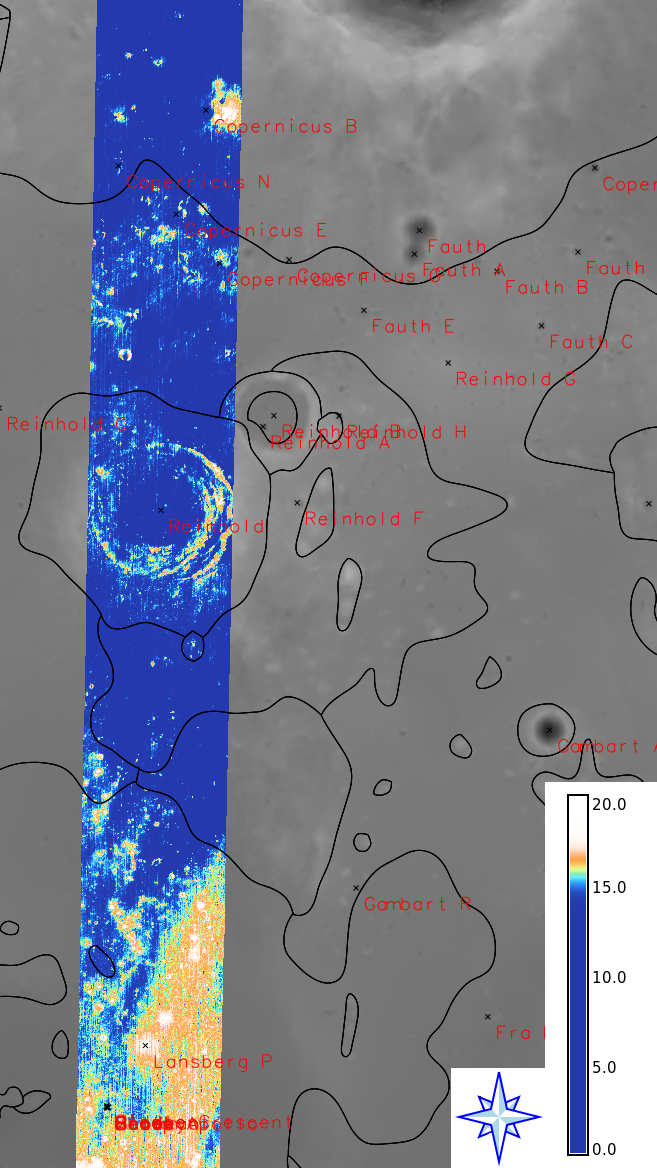
\includegraphics[width=0.45\textwidth,keepaspectratio=true]{./images/M3_Zhang_FeO_region}
% \caption{Region of $M^3$ FeO using \cite{zhang2013mapping} corrected}
 \label{fig:subfeoM3corr}
 Figure 6: Region of $M^3$ FeO using \cite{zhang2013mapping} corrected.
  \end{tabular}
\end{tabular}
\end{center}
\vspace{2mm}
}




\startthirdcolumn
%%%%%%%%%%%%%%%%%%%%%%%%%%%%%%%%%%%%%%%%%%%%%%%%%%%%%%%%%%%%%%%%%%%%%%%%%%%%%%%
\blocknode{Lava Flow Depth}{
\smallskip

\noindent Isolating the 95\% top and 5\% bottom of the destriped FeO image brought the possibility to suggest the Fresh Crater Ejecta (FCE) values. The FCE was found near Lansberg P in the surroundings of (-22.8215621403E,-2.09875487116N) with 11 samples averaging to 17.87 FeO wt\%.\newline 

\begin{center}
	\begin{tabular}{cc}
		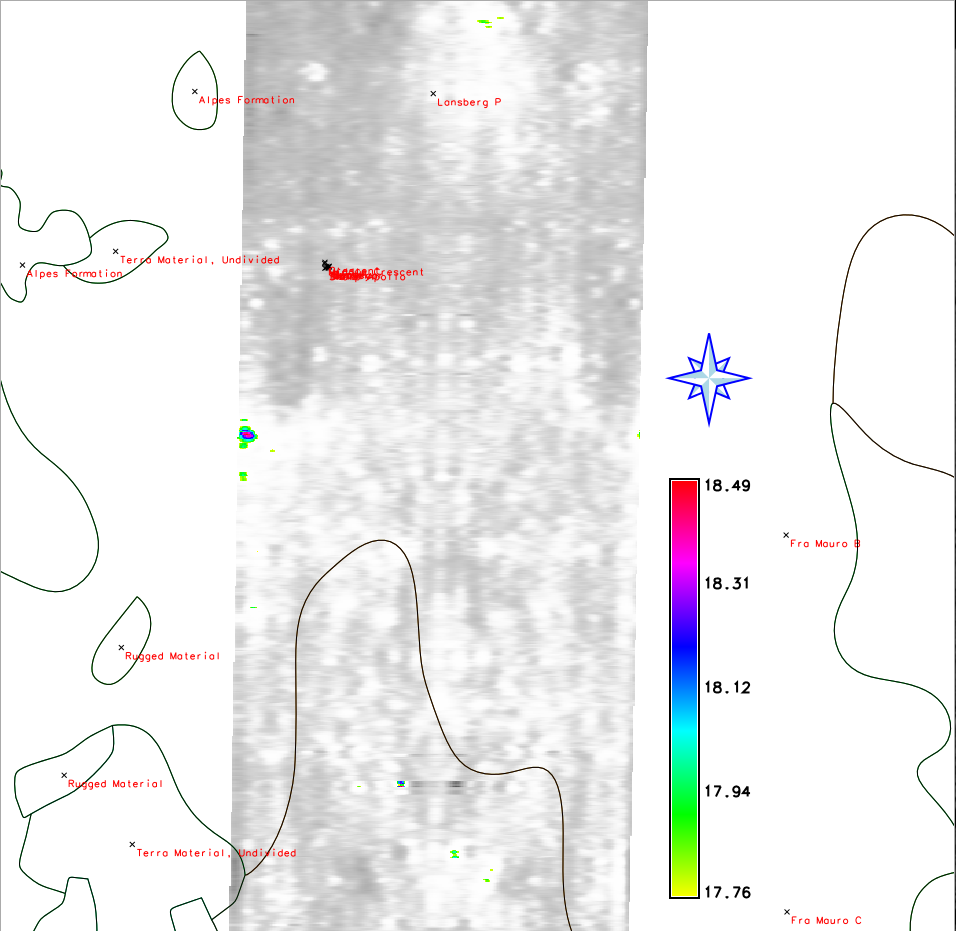
\includegraphics[width=0.42\textwidth]{./images/mdi_high}\hspace{20mm}
		&
		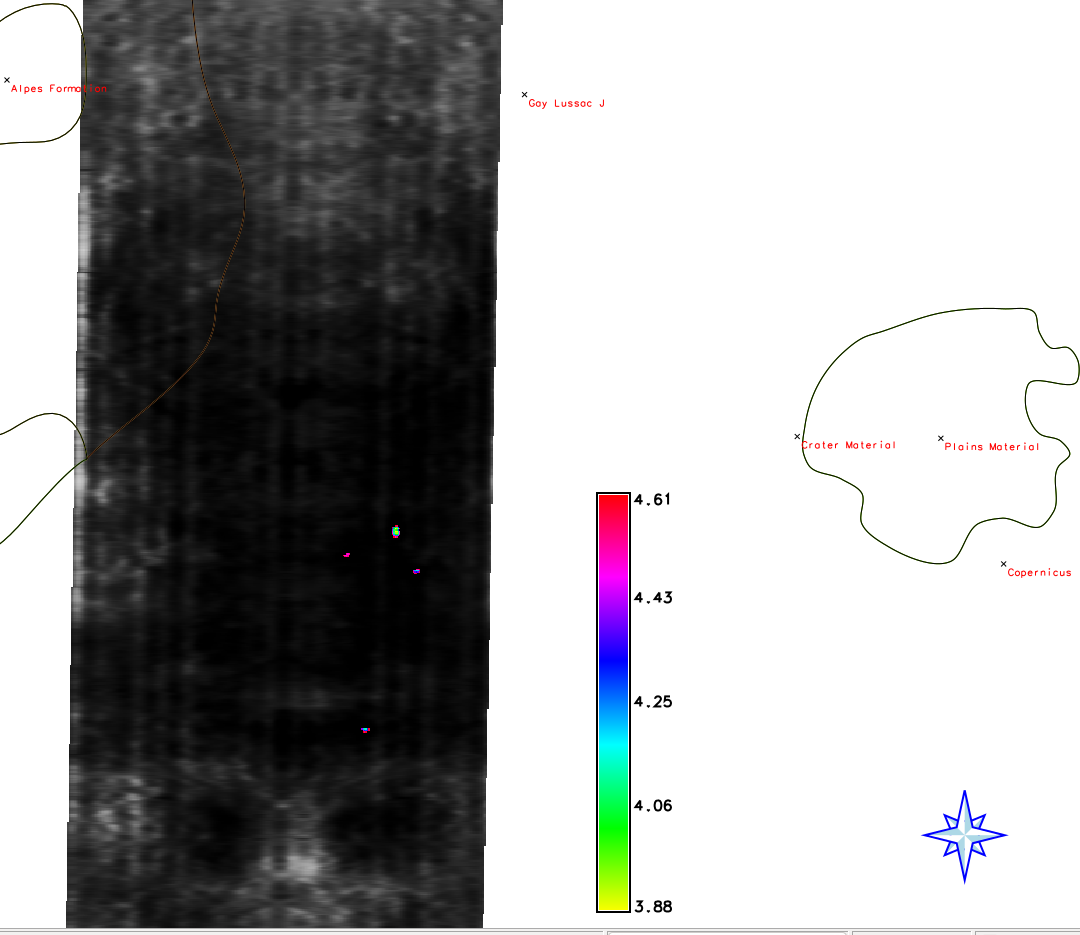
\includegraphics[width=0.47\textwidth]{./images/mdi_low}
	\end{tabular}\newline
Figure 3 (left): Locating FCE above Lansberg P, with the upper 95\% FeO wt\%\\
Figure4 (right): Locating lowest E Westward Copernicus, with the lower 5\% FeO wt\%.
\end{center}

\noindent The H value is the lower boundary of the FeO wt\% in the region, typically found in the nearest highland region. There are two solid constraints to it value. H should be strictly less than E and strictly more than zero ($0<H<E$). The E value was found in Copernicus ejecta ring and actually taken from the FeO wt\% map. The minimum value found in the FeO\_M3G20090111T013904.destripe map is 3.88 wt\%, belonging to the ejecta ring of Copernicus. Thus it can be inferred that $0<H<3.88$, strictly, in this Copernican work. Looking at over M$^3$ FeO tiles, there is no lower value to the crater ejecta of Copernicus. Some Alpes Formation and Dark Mantling Material in the vicinity of Gay Lussac do not go lower than this.\newline

\noindent This is obviously shows the limit of this statistical search method. Another attempt was undertaken using the original tile FeO\_M320090610T113334 a visual search for H in the vicinity of Montes Carpatus (Northwestern of Copernicus with -23.6070634574E, 14.571534275N) was done and from 14 samples found $\overline{H}=5.88$. Another visual search in the ejecta blanket of Copernicus for a FCE value, 22 samples were collected, giving an average FCE value of 7.16. Thus, it is found that $0 < \overline H < \overline{FCE}$, which is a logical outcome. It is thus proposed to carry forward this parametrisation for mapping the depth of the Copernican lava flow with the following equation ~\ref{eq:NewMareDepthVal}.\newline
\begin{equation}\label{eq:NewMareDepthVal}
Mh = \frac {D_*} {8} \times \frac {E-\overline{H}} {\overline{FCE}-\overline{H}} = \frac {117000}{8} \times \frac {E-5.88}{17.87-5.88} [m]
\end{equation}
\noindent Which realizes as the following equation.\newline
\begin{equation}\label{eq:NewMareDepthValCoef}
Mh = (E-5.88) \times 1219.77 [m]
\end{equation} 
}





\blocknode{Conclusions}{
\smallskip
Conclusions
}

\startfourthcolumn
%%%%%%%%%%%%%%%%%%%%%%%%%%%%%%%%%%%%%%%%%%%%%%%%%%%%%%%%%%%%%%%%%%%%%%%%%%%%%%%%
\blocknode{Clementine data}{
\smallskip

\begin{center}
 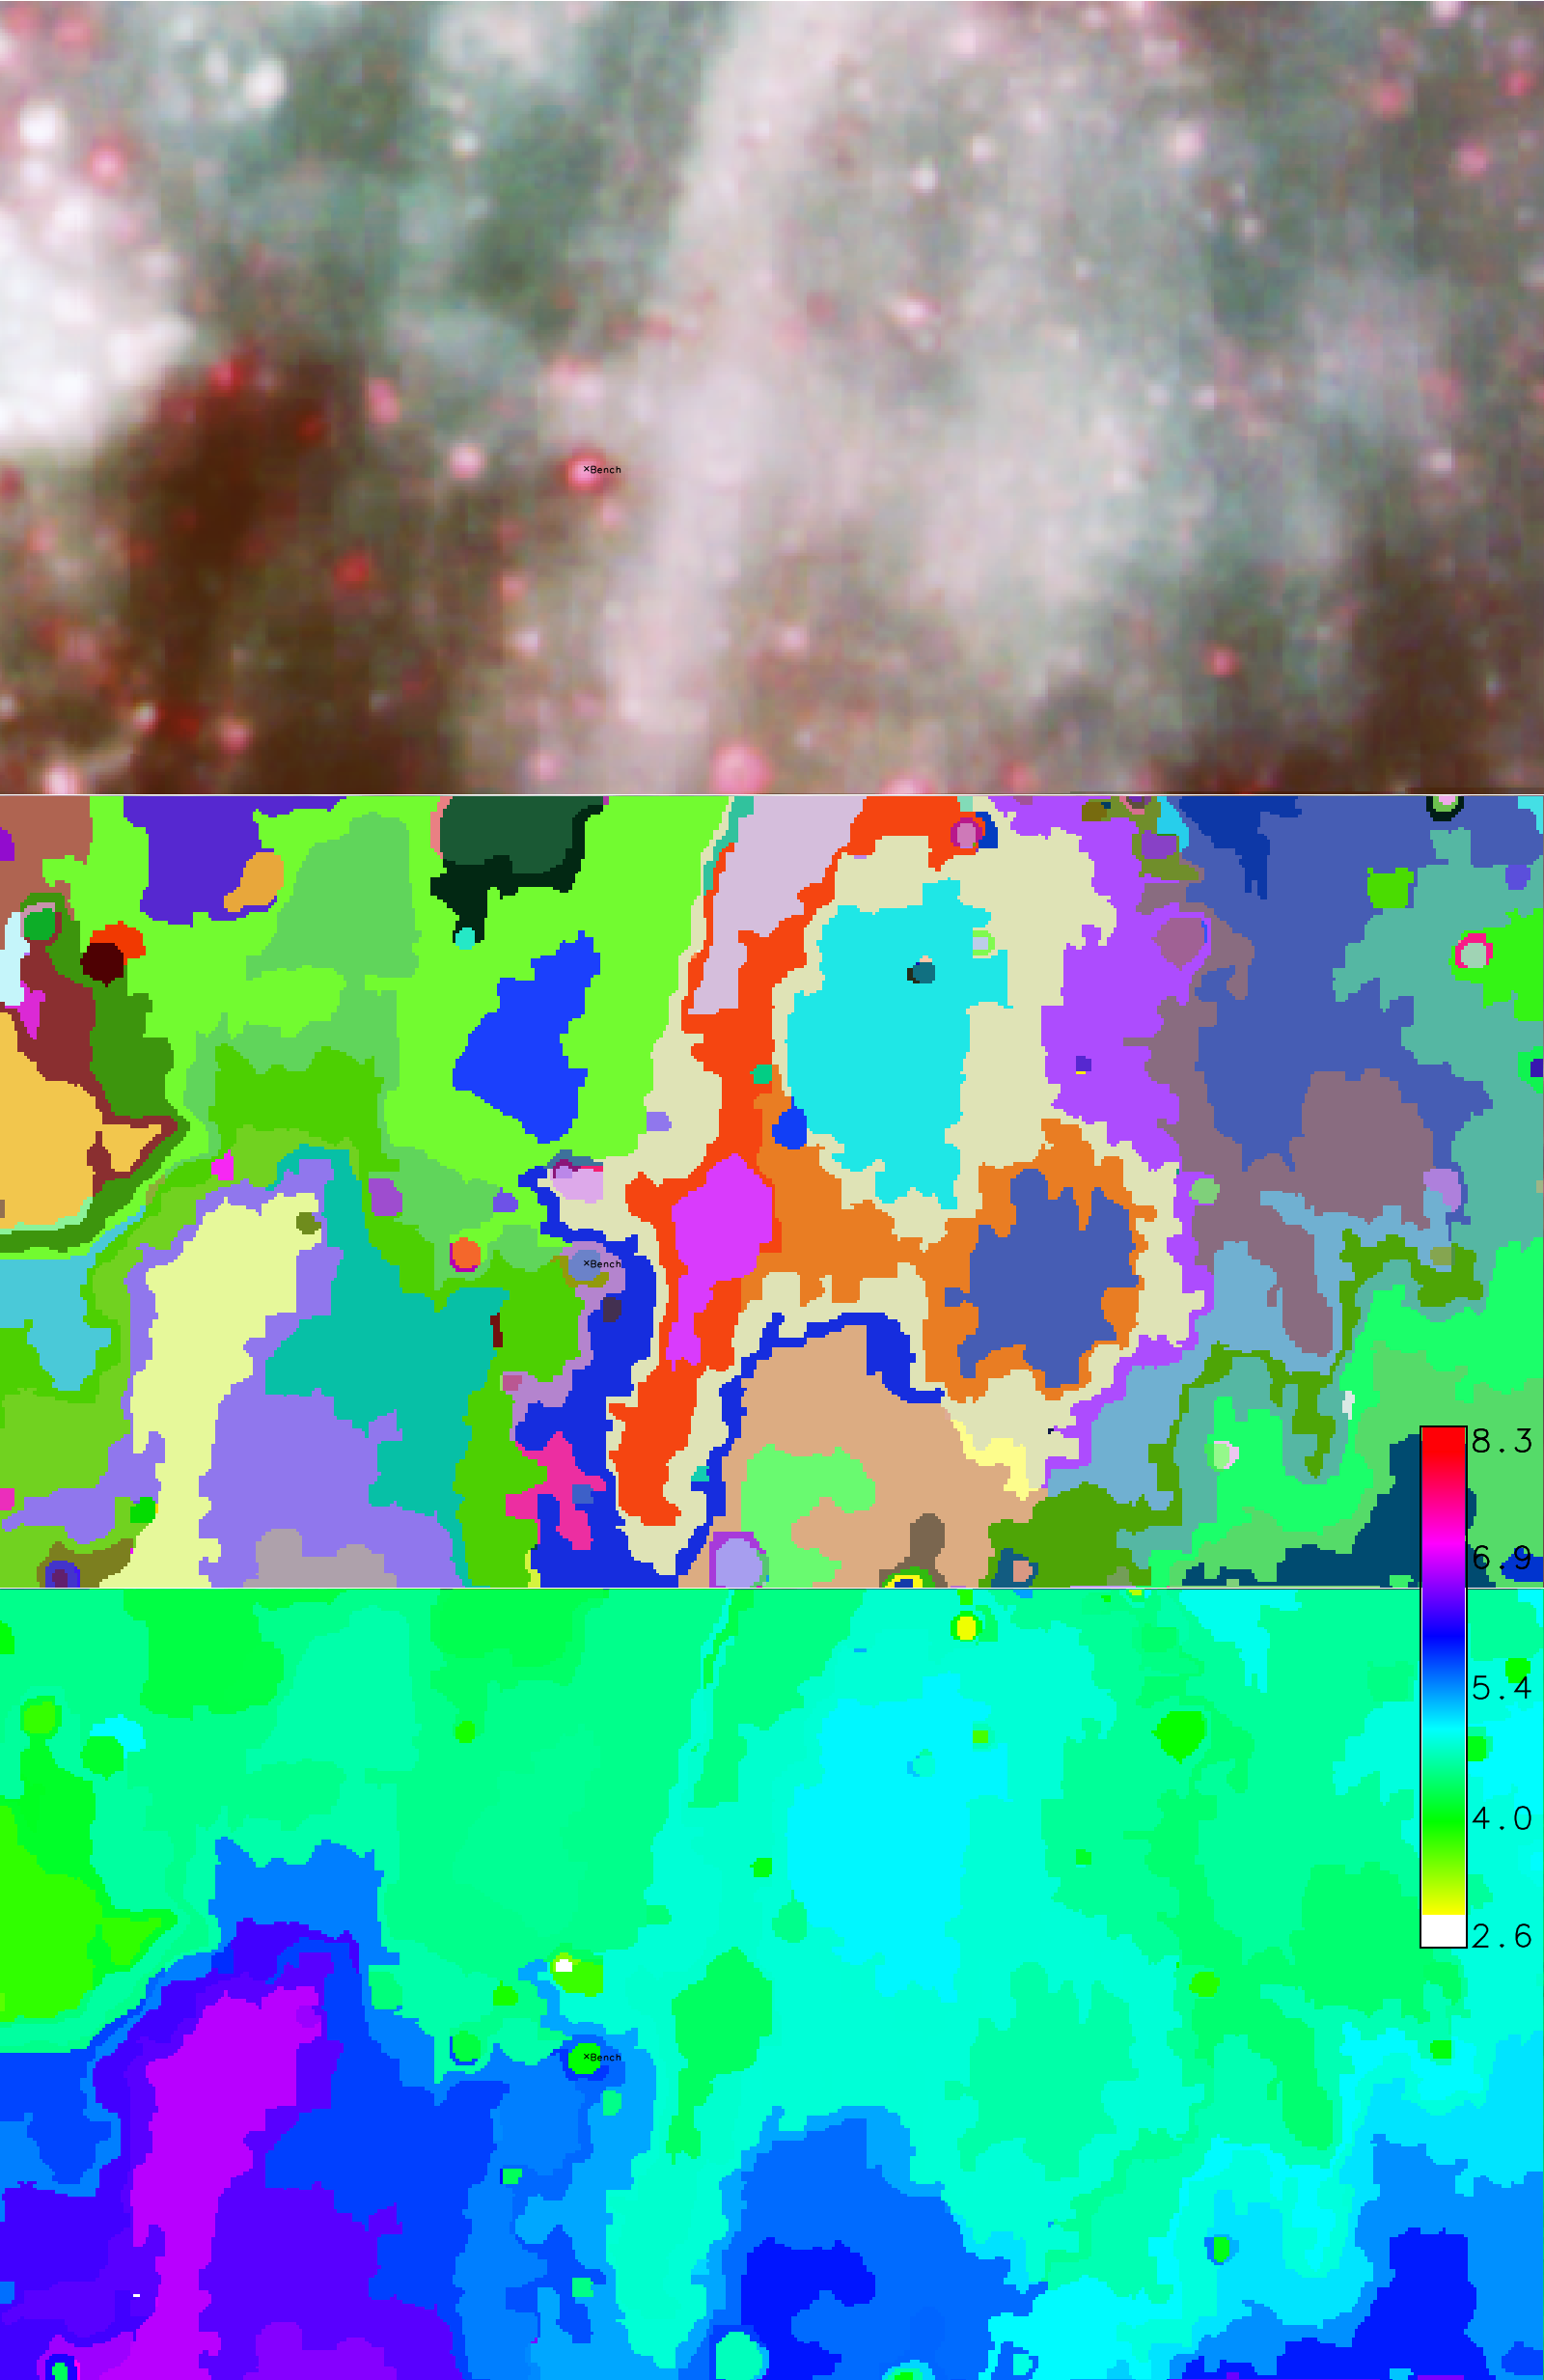
\includegraphics[width=0.45\textwidth]{./images/Clementine}
 \newline
 Figure 3: Clementine RGB153 (top), segmentation (middle) and FeO (wt\%) per segmentation class (bottom).
\end{center}
}
%%%%%%%%%%%%%%%%%%%%%%%%%%%%%%%%%%%%%%%%%%%%%%%%%%%%%%%%%%%%%%%%%%%%%%%%%%%%%%%
\blocknode{M$^3$ Signal at Apollo 12 landing site}{
\smallskip
\begin{center}
\begin{tabular}{ c p{0.45\textwidth} }
 \raisebox{-0.40\totalheight}{ 
 \begin{tabular}{ c }
 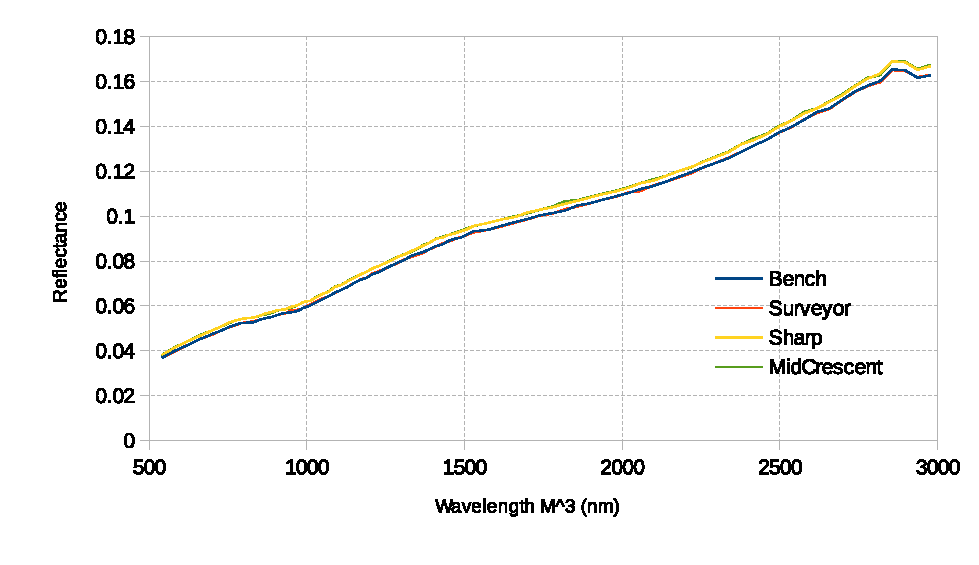
\includegraphics[width=0.5\textwidth]{./images/M3_A12_craters_signal}
  \label{fig:specsignature4craters}\\
  \vspace{5mm}
  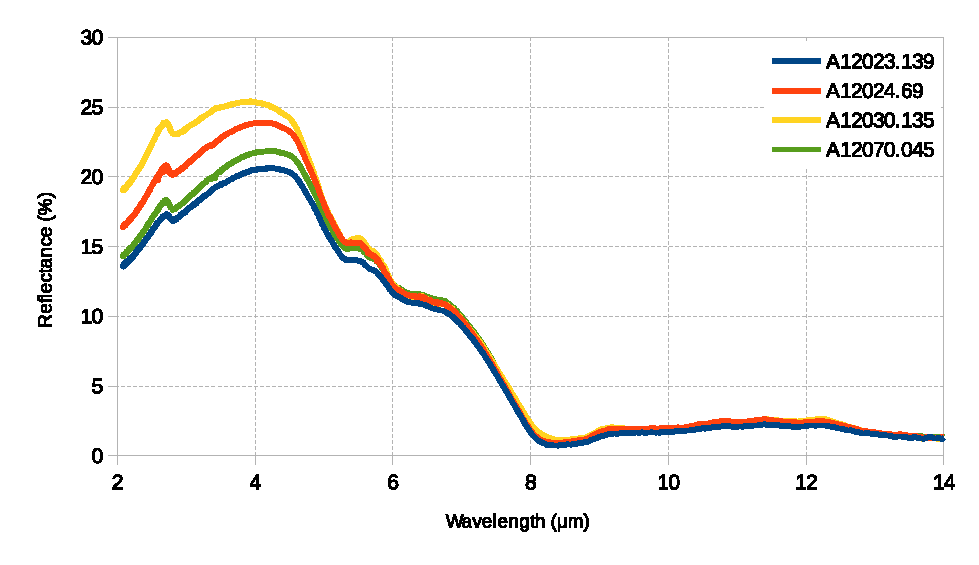
\includegraphics[width=0.5\textwidth]{./images/A12_spectrum}
  \label{fig:specsignaturespeclibv2}\\
  \vspace{5mm}
  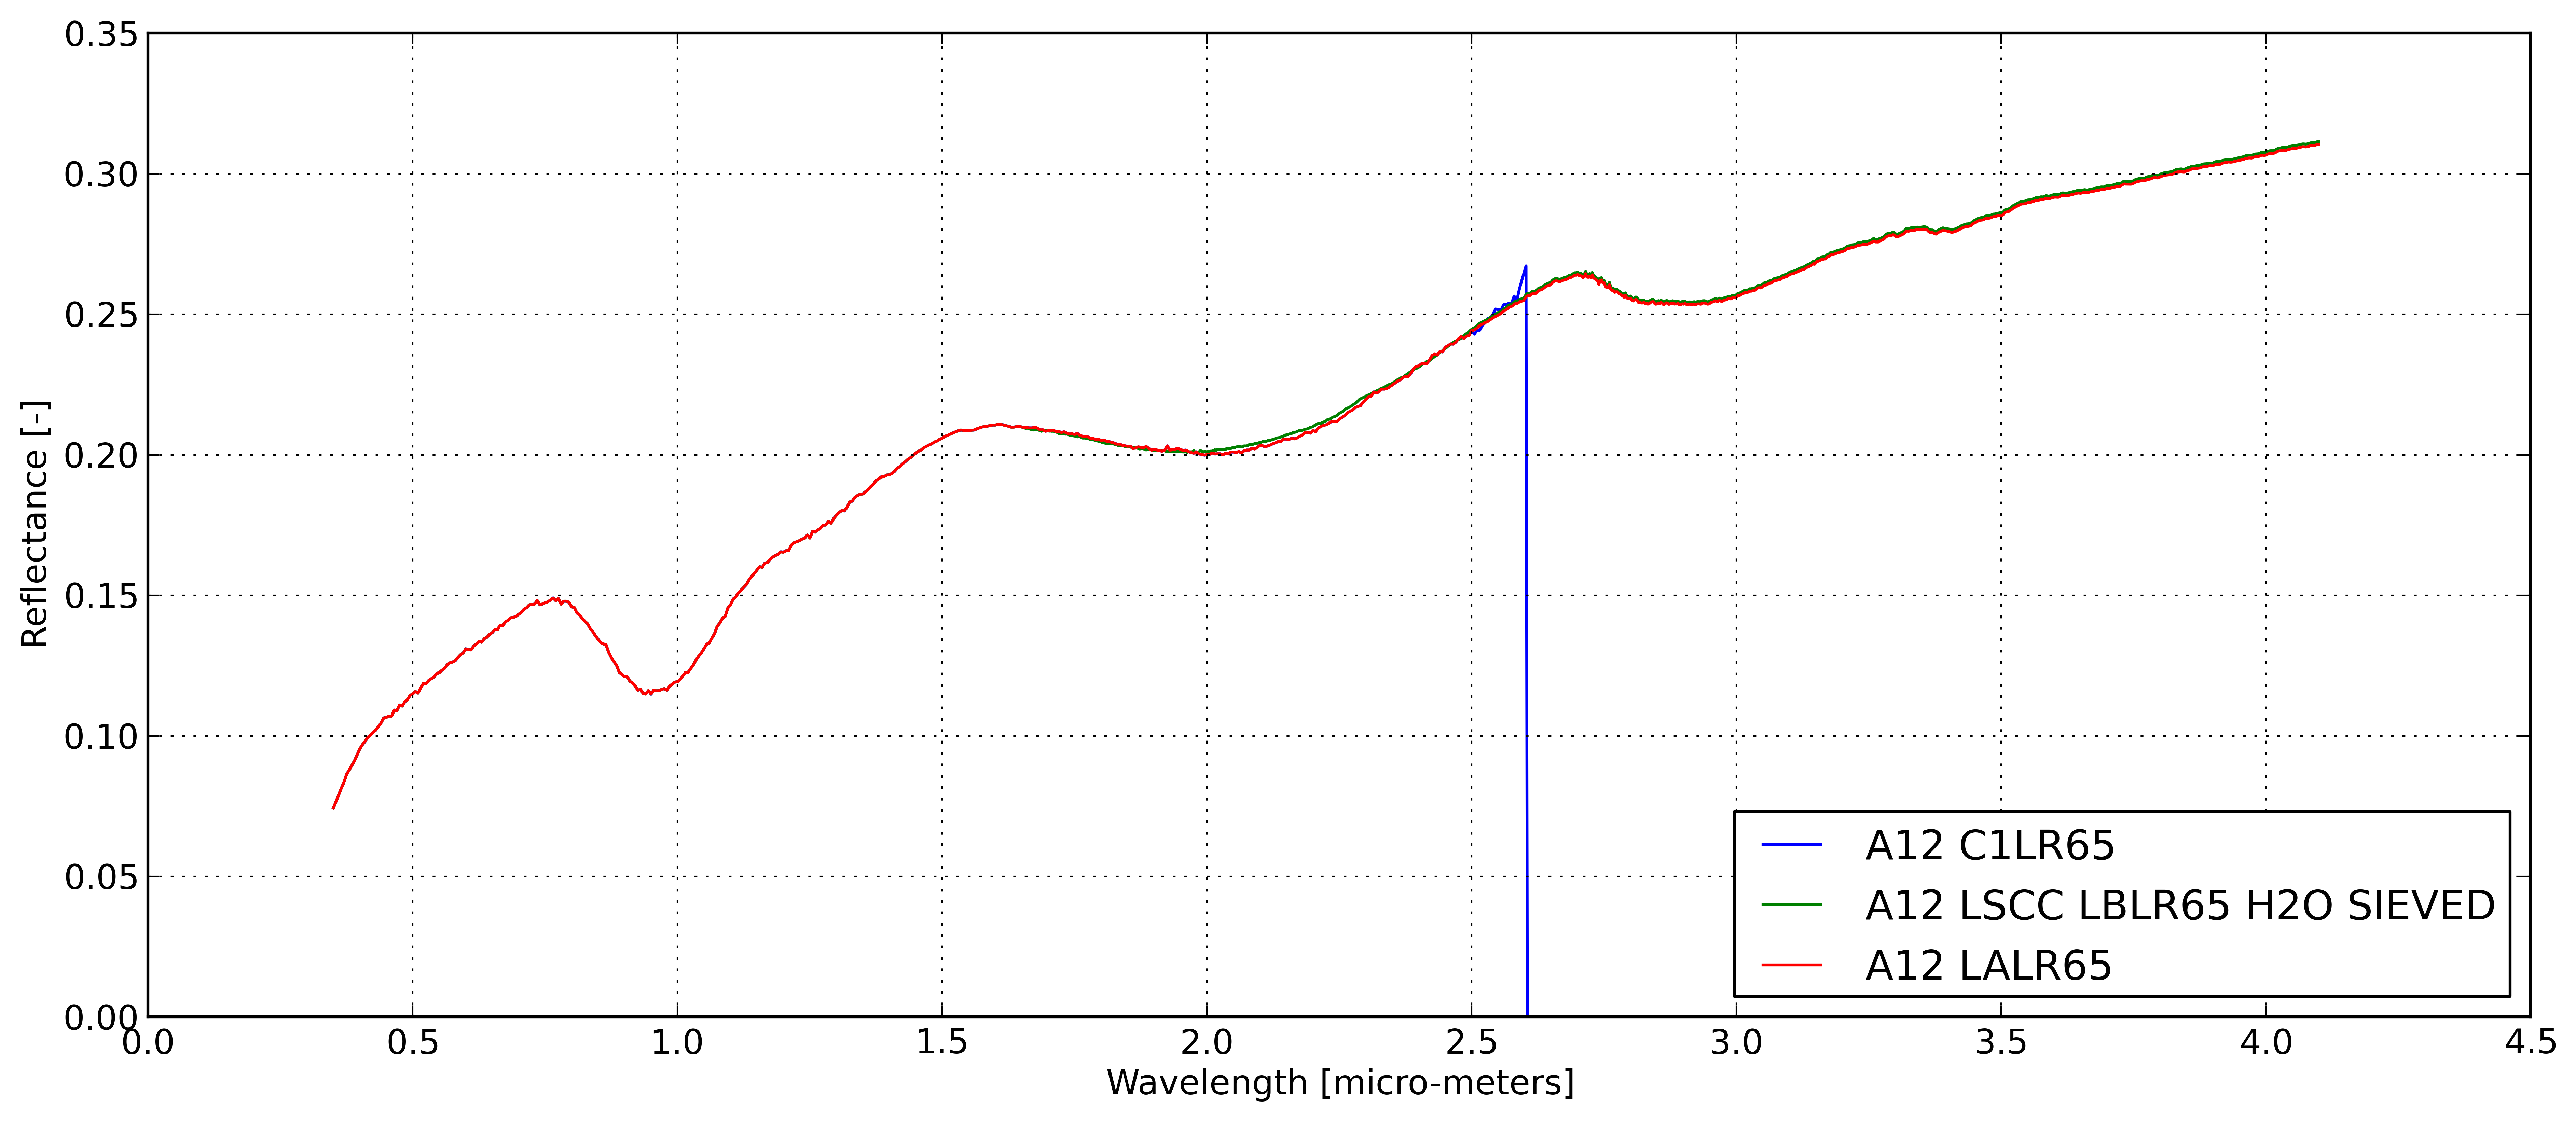
\includegraphics[width=0.5\textwidth]{./images/Apollo12_signatures}
  \label{fig:specsignatureASTERlib}
 \end{tabular} 
 }%End of tabular
 &
 \noindent Chandrayaan $M^3$ data was  downloaded from PDS \url{http://pds-imaging.jpl.nasa.gov/}. The tile \textit{M3G20090111T013904\_V01\_RFL.IMG} was imported in GRASS GIS, resulting in 85 bands. The spectrum for four craters where extracted in the Figure \ref{fig:specsignature4craters}. Bench and Surveyor are both together in the lower reflectance curves. On the higher side, Sharp and Middle Crescent are consistently above the two others. This higher broadband Albedo is increasing towards the West, where one of the ray is clearly drawn (Oblique white strip in the middle of The Clementine upper map. Compared to the spectral data from Figure ~\ref{fig:specsignatureASTERlib} the reflectance is overall lower and the obvious shape differences are there. Additional spectrum signature data from \cite{clark2007usgs} is in the process of being extracted for analysis.\newline\linebreak
 \noindent Figure 8: \newline Spectral signature of $M^3$ from four craters.
 \newline\linebreak 
 \noindent Figure 9: \newline Spectral signature from Apollo 12 (Speclib v2.0).
 \newline\linebreak 
 \noindent Figure 10: \newline Spectral signature from Apollo 12 from \cite{Baldridge2009711}.
 \newline\linebreak 
\end{tabular}
\end{center}
}%End of Block



\end{tikzpicture}

\end{document}
